%% Начало содержательной части.
\chapter{Глава 1. Обзор предметной области}
В данной главе описаны основные понятия и определения из области построения маршрутов в теории графов. В первом разделе главы описаны понятия из теории графов. Во втором разделе описаны понятия из формальной области транспортных сетей. В третьем разделе формализуется задача и список требований по поддерживаемым свойствам для построения маршрутов. Четвертый раздел содержит краткое описание основных алгоритмов теории графов для построение путей со сводной таблицей преимуществ и недостатков данных подходов.

\section{Основные определения}
\begin{definition}
Теория графов -- раздел дискретной математики, изучающий свойства графов.
\end{definition}

\begin{definition}
Граф -- это множество вершин(узлов), соединенных ребрами. В строгом определении графом называется такая пара множеств. $G=(E, V)$, где $V$ есть подмножество любого счетного множества, а $E$ -- подмножество $V \times V$.
\end{definition}

\begin{definition}
Маршрут -- это конечная последовательность вершин, в которой каждая вершина (кроме последней) соединена со следующей в последовательности вершиной ребром. Цепью называется маршрут без повторяющихся рёбер. Простой цепью называется маршрут без повторяющихся вершин (откуда следует, что в простой цепи нет повторяющихся рёбер).
\end{definition}

\begin{definition}
Ориентированный маршрут (или путь) -- это конечная последовательность вершин и дуг, в которой каждый элемент инцидентен предыдущему и последующему.
\end{definition}

\begin{definition}
Цикл -- это цепь, в которой первая и последняя вершины совпадают. При этом длиной пути (или цикла) называют число составляющих его ребер. Заметим, что если вершины и являются концами некоторого ребра, то согласно данному определению, последовательность является циклом. Чтобы избежать таких «вырожденных» случаев, вводят следующие понятия.
\end{definition}

\begin{definition}
Транспортное средство -- это совокупность технических систем, предназначенных для перемещений людей и грузов из одного места в другое.
\end{definition}

\begin{definition}
Транспортный узел -- это комплекс транспортных устройств в пункте стыка нескольких видов транспорта, совместно выполняющих операции по обслуживанию транзитных, местных и городских перевозок грузов и пассажиров.
\end{definition}

\begin{definition}
Транспортный рейс --
\end{definition}

\begin{definition}
Транспортная сеть -- это совокупность всех транспортных рейсов, представленных в течение интервала продажи билетов.
\end{definition}

\begin{definition}
Остановка — специально отведенное общественное место, предназначенное для посадки/высадки пассажиров рейсового транспортного средства.
\end{definition}

\begin{definition}
Расписание — 
\end{definition}

\begin{definition}
Мульмодальный маршрут — это конечная последовательность транспортных рейсов, попав на которые в определенные промежутки времени можно добраться от начального транспортного узла до конечного.
\end{definition}

\begin{definition}
Построитель маршрутов — это программный комплекс для обработки внешних поисковых клиентских запросов, имеющий доступ к полному объему данных о расписаниях на всех транспортных узлах и осуществляющий выдачу определенного количества маршрутов в соответствии с поступившими в запросах требованиями. Также в качестве дополнительных возможностей доступно построение фильтров и различной статистики (активные транспортные узлы, активные транспортные рейсы, проходящие через заданный узел).
\end{definition}

\begin{definition}
Клиентское приложение — это любое приложение, которое осуществляет запросы к построителю маршрутов за результатом (маршрутами и фильтрами).
\end{definition}

\section{Виды транспорта и его особенности}
В транспортной сети, в которой будут строиться маршруты, будет существовать только транспорт с конкретным расписанием транспортных рейсов. Таким образом, идет допущение о том, что система сети идеальна и весь транспорт гарантировано совершает остановки в назначенное время. Постановка вспомогательных свойств для построителя маршрутов, которые позволяют сгладить последствия этого допущения будут описаны в следующих главах. Далее идет описание рассматриваемого транспорта.

\subsection{Железнодорожный}
В задаче будут рассматриваться 2 вида железнодорожного транспорта. Во-первых, это будут поезда дальнего следования, у которых небольшое количество рейсов (около $10^5$ в течение интервала продажи билетов). Во-вторых, это будут электрички, которые уже совершают до $10^6$ рейсов за аналогичный промежуток времени.
Транспортными узлами являются железнодорожные станции и вокзалы.

\subsection{Воздушный}
Воздушный транспорт будет представлен только самолетами. При этом количество рейсов около $10^3$, поэтому особый интерес этот случай не представляет. Но стоит отметить, что в большинстве случаев мультимодальный маршрут не будет содержать больше одного воздушного сегмента пути.
Транспортными узлами являются аэропорты.

\subsection{Автомобильный}
Автомобильный транспорт состоит из автобусных междугородних рейсов. Около 95\% таких рейсов совершаются только между соседними городами, что сильно упрощает задачу, но количество все равно большое — $10^6$.
Также в эту категорию входит транспорт в пределах города (или любого крупного населенного пункта), например, такси. Стоит отметить, что в этот вид транспорта можно внести любые другие средства передвижения внутри города, так как в конечном счете это не будет влиять на алгоритм. При этом важно, чтобы у нового транспорта в пределах города имелась возможность рассчитать эвристическое времени передвижения между двумя транспортными узлами, которые относятся к одному населенному пункту. Эту задачу следует решать на основе статистики или с помощью сторонних сервисов, которые умеют анализировать дорожную ситуацию, например, такие сервисы, как 2gis или Яндекс.карты, которые могут оценить время движения на основе карты пробок.
Транспортными узлами являются автобусные остановки и крупные населенные пункты.

\section{Построение маршрутов}
Основная задача, ставящаяся перед построителем маршрутов — построение маршрутов по данным, доступным в его памяти и внешних базах данных, доступных для чтения в конкретный момент времени. На алгоритм построения маршрутов в транспортной сети накладываются следующие условия и ограничениями.

\subsection{Мультимодальность}
Маршруты могут быть мультимодальными, то есть проходить через несколько точек-остановок, содержать пересадки, проходить разными видами транспорта со своими особенностями и т.д.; Это нужно для того, чтобы была возможность добраться из любой точки в любую, где есть хотя бы какой-нибудь транспорт. Вариант пройти пешком небольшой кусок пути тоже доступен внутри крупного населенного пункта также должен быть доступен.
\begin{figure}[!h]
    \centering
    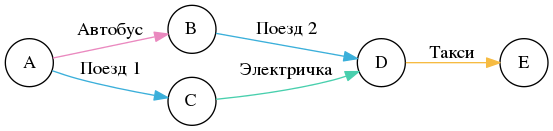
\includegraphics[width=\textwidth]{multimodal_example.png}
    \caption{Несколько мультимодальных маршрутов от точки A до точки E.}\label{fig1}
\end{figure}

\subsection{Временные интервалы}
Маршруты можно строить для определенных интервалов времени. Например, хотим выехать в промежуток с 8-00 до 12-00 утра, а приехать в любой день на следующей неделе, но обязательно после 21-00. Это требуется, чтобы иметь возможность бронировать гостиницу, не отходя от кассы.

\subsection{Инкрементальное построение}
Маршруты требуется строить инкрементально (не все сразу, а только небольшую часть из существующих) из-за того, что возможное количество маршрутов может достигать до 109 между парой крупных населенных пунктов с 3 допустимыми пересадками и интервалом времени в пути равным нескольким дням. Это требуется для конечного клиентского приложения, чтобы можно было организовать страничный показ результатов без полного вычисления всех маршрутов на предыдущих страницах.

\subsection{Адаптивность по времени}
Маршруты могут строиться адаптивно по времени из-за того, что важно время отклика алгоритма, то есть в приоритете время выполнения над показом действительно всех требуемых результатов.

\section{Построение фильтров к доступным маршрутам}
Под фильтром в данном случае понимается предикат, который принимает в качестве аргумента построенный маршрут и возвращает ИСТИНА или ЛОЖЬ в зависимости от того, удовлетворяет ли маршрут критериям поиска, которые задает фильтр.
Таким образом, помимо построения самих маршрутов требуется построить фильтры по доступным маршрутам со следующими условиями.

\subsection{Косвенные признаки}
Из-за того, что маршруты строятся не все сразу, то кроме непосредственно найденных маршрутов существует огромное количество потенциально доступных маршрутов. При этом мы хотим получить к ним доступ по косвенным признаками. Например, это может быть тип транспорта, номер поезда или тип места в самолете (у окна/у туалета/в хвосте). Формально любой параметр доступный в модели данных может стать доступным для фильтрации.
Примечание. Под моделью данных в данном случае подразумевается любой абстрактный объект, который имеет отражение в реальном мире: поезд, самолет, аэропорт и т.д.

\subsection{Осуществление фильтрации}

\subsection{Функциональные зависимости}
Не последнюю роль в фильтрах играют функциональные зависимости, потому что в последствии нужно будет их эффективно показывать без противоречий. Например, тип места «у окна» в купе и каюте относятся к разным типам транспорта и их нельзя объединять. Пример «дерева» функциональный зависимостей для поезда:
\begin{itemize}
    \item Точки отправления и прибытия
    \item Интервалы отправления и прибытия
    \item Вид транспорта:
    \item Поезд:
    \item Перевозчик
    \item Бренд
    \item Номер
    \item Тип вагона:
    \item Купе:
    \item Верхнее/нижнее
    \item Не у туалета
    \item Сидячий:
    \item У окна/у прохода
    \item Плацкарт:
    \item Верхнее/нижнее
    \item Не у туалета
    \item Боковое/не боковое
\end{itemize}

Каждый уровень списка зависит от родительского уровня и строго им определяется для того, чтобы исключить ситуации, когда несколько косвенных признаков совпадают уже разных видов транспорта. Например, признак «Перевозчик» у поезда и самолета. Такое разделение необходимо для корректного с точки зрения логики и удобного вывода результата в клиентском приложении.

\section{Сортировка маршрутов}
Маршруты требуется строить в порядке сортировки. В простейшем варианте можно сортировать только построенные маршруты, что не представляет из себя никакой сложности. В сложном варианте маршруты строятся на основе любого предиката сравнения пары маршрутов и выдаются в результат, гарантируя определенный порядок. В рамках данной работы подходит «средний» вариант. Требуется гарантировать определенный порядок построенных маршрутов без пропусков, но предикаты известны заранее. Всего их основных 4 вида:
\begin{enumerate}
    \item Количество пересадок
    \item Время отправления
    \item Время прибытия
    \item Время в пути
\end{enumerate}

Рассмотрим каждый подробнее.

\subsection{Количество пересадок}
Самая простая сортировка в рамках данной работы (или просто сортировка по-умолчанию). Несложно заметить, что количество пересадок будет пропорционально количеству транспорта, который будет включен в мультимодальный маршрут. И если представить каждый отрезок пути на конкретном транспорте отдельным ребром в абстрактном графе, то сортировка будет происходить относительно количества ребер.
\subsection{Время отправления}

\subsection{Время прибытия}

\subsection{Время в пути}

\section{Известные алгоритмы}
\subsection{Алгоритм Дейкстры}
Алгоритм Дейкстры - алгоритм на графах, изобретённый нидерландским учёным Эдсгером Дейкстрой в 1959 году. Находит кратчайшие пути от одной из вершин графа до всех остальных. Алгоритм работает только для графов без рёбер отрицательного веса.

\section{Таблицы}

В качестве примера таблицы приведена таблица~\ref{tab1}.

\begin{table}[!h]
\caption{Таблица умножения (фрагмент)}\label{tab1}
\centering
\begin{tabular}{|*{18}{c|}}\hline
-- & 1 & 2 & 3 & 4 & 5 & 6 & 7 & 8 & 9 & 10 & 11 & 12 & 13 & 14 & 15 & 16 & 17 \\\hline
1  & 1 & 2 & 3 & 4 & 5 & 6 & 7 & 8 & 9 & 10 & 11 & 12 & 13 & 14 & 15 & 16 & 17 \\\hline
2  & 2 & 4 & 6 & 8 & 10 & 12 & 14 & 16 & 18 & 20 & 22 & 24 & 26 & 28 & 30 & 32 & 34 \\\hline
3  & 3 & 6 & 9 & 12 & 15 & 18 & 21 & 24 & 27 & 30 & 33 & 36 & 39 & 42 & 45 & 48 & 51 \\\hline
4  & 4 & 8 & 12 & 16 & 20 & 24 & 28 & 32 & 36 & 40 & 44 & 48 & 52 & 56 & 60 & 64 & 68 \\\hline
\end{tabular}
\end{table}

Есть еще такое окружение \texttt{tabu}, его можно аккуратно растянуть на всю страницу.
Приведем пример (таблица~\ref{tab2}).

\begin{table}[!h]
\caption{Таблица умножения с помощью \texttt{tabu} (фрагмент)}\label{tab2}
\centering
\begin{tabu}{|*{18}{X[c]|}}\hline
-- & 1 & 2 & 3 & 4 & 5 & 6 & 7 & 8 & 9 & 10 & 11 & 12 & 13 & 14 & 15 & 16 & 17 \\\hline
1  & 1 & 2 & 3 & 4 & 5 & 6 & 7 & 8 & 9 & 10 & 11 & 12 & 13 & 14 & 15 & 16 & 17 \\\hline
2  & 2 & 4 & 6 & 8 & 10 & 12 & 14 & 16 & 18 & 20 & 22 & 24 & 26 & 28 & 30 & 32 & 34 \\\hline
3  & 3 & 6 & 9 & 12 & 15 & 18 & 21 & 24 & 27 & 30 & 33 & 36 & 39 & 42 & 45 & 48 & 51 \\\hline
4  & 4 & 8 & 12 & 16 & 20 & 24 & 28 & 32 & 36 & 40 & 44 & 48 & 52 & 56 & 60 & 64 & 68 \\\hline
\end{tabu}
\end{table}

\section{Рисунки}

Пример рисунка (c помощью \texttt{TikZ}) приведен на рисунке~\ref{fig1}. Под \texttt{pdflatex} можно также
использовать \texttt{*.jpg}, \texttt{*.png} и даже \texttt{*.pdf}, под \texttt{latex} можно использовать
Metapost. Последний можно использовать и под \texttt{pdflatex}, для чего в стилевике продекларированы
номера картинок от~1 до~20.

\begin{figure}[!h]
\caption{Пример рисунка}\label{fig1}
\centering
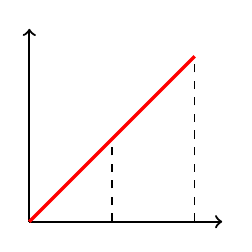
\begin{tikzpicture}[scale=0.7]
\draw[thick,->] (0,0)--(3.5,0);
\draw[thick,->] (0,0)--(0,3.5);
\draw[very thick, red] (0,0)--(3,3);
\draw[dashed] (3,0)--(3,3);
\draw[dashed] (1.5,0)--(1.5,1.5);
\end{tikzpicture}
\end{figure}

\section{Листинги}

В работах студентов кафедры <<Компьютерные технологии>> часто встречаются различные листинги. Листинги бывают
двух основных видов~--- исходный код и псевдокод. Первый оформляется с помощью окружения \texttt{lstlisting}
из пакета \texttt{listings}, который уже включается в стилевике и немного настроен. Пример Hello World на Java
приведен на листинге~\ref{lst1}.

\begin{lstlisting}[float=!h,caption={Пример исходного кода на Java},label={lst1}]
public class HelloWorld {
	public static void main(String[] args) {
		System.out.println("Hello, world!");
	}
}
\end{lstlisting}

Псевдокод можно оформлять с помощью разных пакетов. В данном стилевике включается пакет \texttt{algorithmicx}.
Сам по себе он не генерирует флоатов, поэтому для них используется пакет \texttt{algorithm}.
Пример их совместного использования приведен на листинге~\ref{lst2}. Обратите внимание, что флоаты разные, а 
нумерация~--- общая!

\begin{algorithm}[!h]
\caption{Пример псевдокода}\label{lst2}
\begin{algorithmic}
	\Function{IsPrime}{$N$}
		\For{$t \gets [2; \lfloor\sqrt{N}\rfloor]$}
			\If{$N \bmod t = 0$}
				\State\Return \textsc{false}
			\EndIf
		\EndFor
		\State\Return \textsc{true}
	\EndFunction
\end{algorithmic}
\end{algorithm}

Наконец, листинги из \texttt{listings} тоже можно подвешивать с помощью \texttt{algorithm},
пример на листинге~\ref{lst3}.

\begin{algorithm}[!h]
\caption{Исходный код и флоат \texttt{algorithm}}\label{lst3}
\begin{lstlisting}
public class HelloWorld {
	public static void main(String[] args) {
		System.out.println("Hello, world!");
	}
}
\end{lstlisting}
\end{algorithm}
